% D06-001. PDR-05, таблицы 5/6/10, рисунок 7.
\section{Первые результаты сопоставления аналитических органов}
\label{sec:ch5_first_results}
\conceptsource{Статья 5, массовая статистика и экспертная
проверка аналитических РНМ. Числа перенесены из снимка статьи.
Они не являются новым пересчётом продолжающейся разметки.}

Результаты далее отвечают на три последовательных вопроса.
Где органы расходятся между собой, какие различия связаны
с составом архивов и какой ответ подтверждается экспертным просмотром.
Матрица согласия нужна для поиска похожих и различающихся органов,
а не для выбора правильного ответа большинством голосов.
Для объяснения отдельного расхождения требуется вернуться к записи.
Сводные показатели рассматриваются вместе с осциллограммами
в подразделе~\ref{sec:ch5_waveform_cases}.

\subsection{Распределение состояний и область малых токов}
\conceptsource{Статья 5, подразделы 7.2--7.3.
Распределение выходов отличается от точности,
а токовая группа относится к записи в целом.}

\iffalse
(Примечание автора: Распределительном? Это каком? Не понял термина.)
(Примечание автора: Ок, закрываем задачу.)
\fi
\authorreviewnote{AA172}

В архиве Open\_EE средняя пофайловая доля
прямого выхода адаптивного органа составила 59,15\%.
Для пофазного углового получено 42,66\%,
для углового прямой последовательности 50,11\%.
Во French/RTE соответствующие доли равны
52,16, 47,32 и 53,10\%.
Это распределение состояний органов,
а не доли правильных решений.
По большему числу блокирующих ответов
нельзя заключить, что орган лучше различает режимы.

Более содержательную картину даёт разбиение
по характерному току осциллограммы.
Для каждой записи рассчитывается действующий ток,
затем используется медиана по доступным фазам.
Полученная величина характеризует файл целиком.
Она не является мгновенным током
в каждой точке последующего расхождения.

В Open\_EE группа от 0,01 до
$0{,}05I_{\text{ном}}$ содержит 14,85\% записей.
Средняя пофайловая доля разногласий девяти органов
в этой группе составляет 52,25\%.
Доля прямого ответа адаптивного органа здесь
равна 55,15\%, пофазного углового 2,53\%,
углового прямой последовательности 3,46\%.
Разница порогов 0,01 и 0,05 номинального тока
существенна для рассмотрения этого результата.
Однако одной групповой статистики недостаточно,
чтобы приписать каждое расхождение только уставке.

\begin{figure}[htbp]
\centering
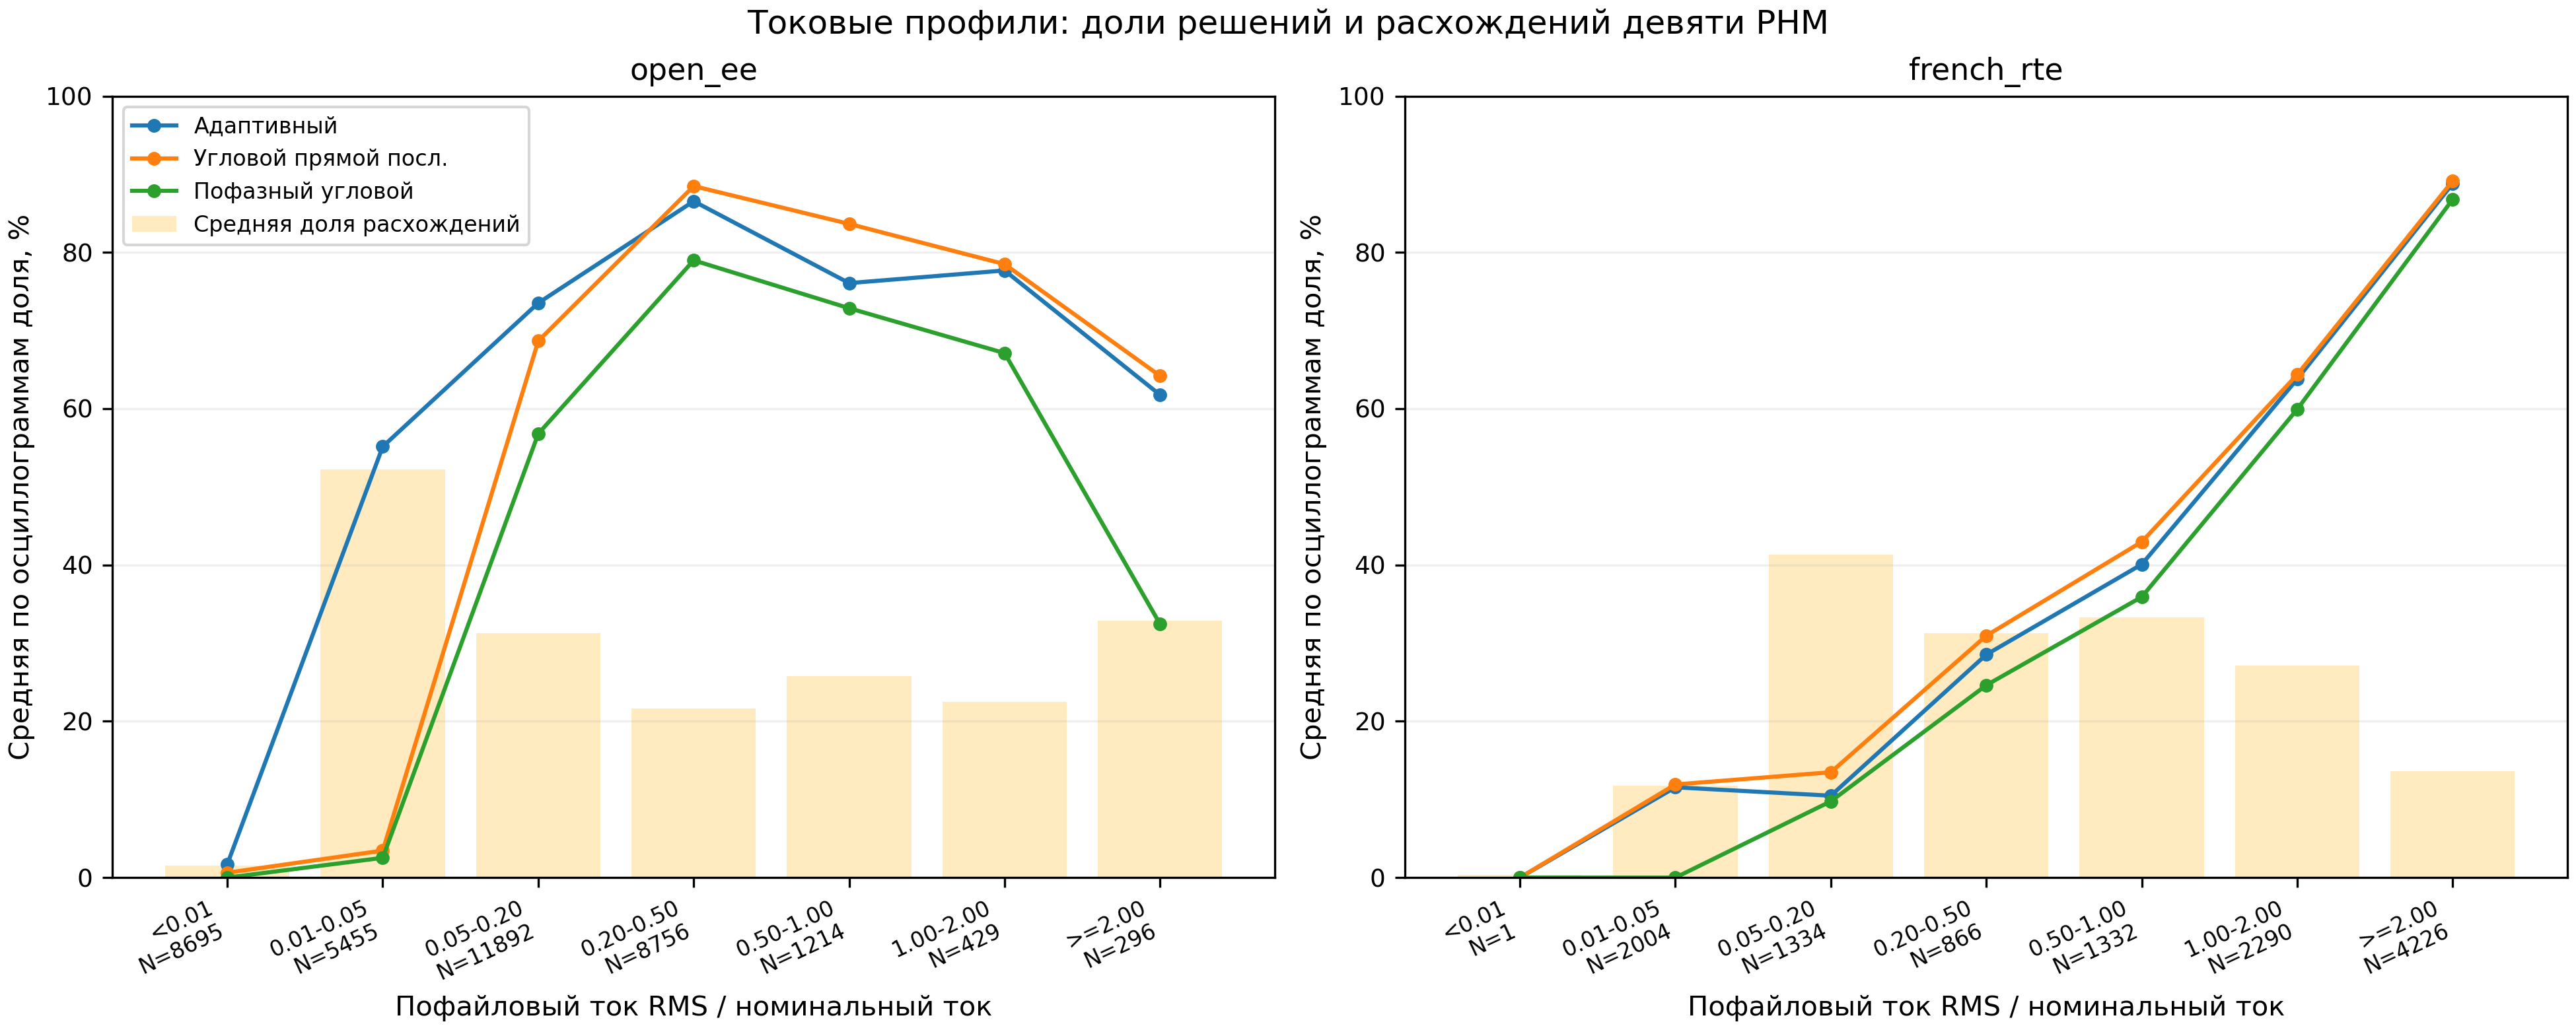
\includegraphics[width=\textwidth]{figures/ch05/ch05_current_profiles_article.png}
\caption{Распределение прямых решений и разногласий
в группах осциллограмм с разным характерным током}
\label{fig:ch5_current_profiles}
\end{figure}
\figurereview{Исходный рисунок 7 статьи 5. При подготовке
к печати увеличить подписи групп и заменить технические
имена источников читаемыми названиями. Число N под интервалом
есть число файлов, а не отсчётов.}

В магистральном архиве структура иная.
Доля записей с характерным током не ниже
двух номинальных составляет 35,06\%,
среднее разногласие внутри этой группы 13,66\%.
В группе 0,05--0,20 номинального тока
оно достигает 41,29\%.
Поэтому общий средний результат
рассматривается вместе с физическим составом источника.

Практическое значение анализа состоит
в выделении области для последующего изменения
и контролируемой проверки характеристики.
Например, сравнение токовых уставок выполняется
при сохранении остальных частей органа.
Иначе одновременно изменённые опорная величина,
память и порог не позволяют выделить
вклад одного принятого решения.

Доля разногласий определяется по тем позициям записи,
где применимы хотя бы два органа. Позиция считается спорной,
если среди их ответов одновременно есть прямое и обратное
направления. Если сравнимых позиций в файле нет, его доля
принимается нулевой. Поэтому среднее по файлам зависит
не только от расхождений, но и от состава таких записей.

% R5-04: закрыто автором 2026-11-11.
\iffalse
% D06-005 R5-04 BEGIN
\ifdefined\AuthorReview
\par\smallskip\begingroup\small\raggedright\color{red!60!black}
\noindent\textbf{Примечание рецензента [R5-04], определение показателя.} Для числа 52,25 процента в предыдущем подразделе явно определить событие разногласия. В сохранённом study.py сравнимы точки, где применимы хотя бы два органа; расхождение означает наличие среди них обоих направлений. При отсутствии таких точек файл получает нулевую долю. Это отличается от общей применимости всех девяти органов в распределении комбинаций ниже и от среднего по 36 парам. Текстовое пояснение генератора о «общих валидных точках» недостаточно точно. Число совпадает со сводкой; уточнить знаменатель и влияние нулевых файлов, не исправляя результат наугад.\par\endgroup\smallskip
\fi
% D06-005 R5-04 END
\ifdefined\AuthorReview
\par\smallskip{\small\color{blue!60!black}\noindent\textbf{Ответ D06-006 на R5-04 (10.11.2026).} Определение проверено по osc\_tools/pdr/study.py: сравнимы позиции хотя бы с двумя применимыми органами, разногласие означает наличие обоих направлений. При отсутствии сравнимых позиций пофайловая доля нулевая. Пояснение добавлено, число сохранено.\par}\smallskip
\fi

(Примечание автора: Ок, обсуждение выше закрываем.)
\fi

\iffalse
(Примечание автора: Вроде слова какие-то есть, но понятности не особо дало. По всему подразделу с графиками, написанно как-то так себе.)
\fi
\authorreviewnote{AA173}

\subsection{Попарное согласие и общие решения органов}
\label{sec:ch5_population_agreement}
\conceptsource{Статья 5, подразделы 6.4, 7.4--7.5,
таблицы 7--8 и рисунки 4--5.
Числа относятся к совместно применимым отсчётам,
а не к равновесному среднему файлов или физического времени.}

Токовые группы локализуют область расхождения,
но не показывают, какие характеристики дают близкие ответы.
Для этого сопоставляются пары органов
на отсчётах их совместной применимости.
В таблице~\ref{tab:ch5_pairwise_disagreement}
приведена доля несовпадающих направлений.
Каждая пара имеет собственный набор применимых отсчётов.
Поэтому её результат нельзя считать оценкой
на одном неизменном для всех органов подмножестве.

\iffalse
(Примечание автора: Вот ты из разу в раз повторяешь про «нельзя считать оценкой на одном неизменном для всех органов подможестве». Ну может не везде такими словами, но прям повторяешь из раза в раз… Ну вот перестань в такие дебри закапываться..)
(Примечание автора: Ок, раз это отдельная задача - то тут закрываем вопрос.)
\fi
\authorreviewnote{AA174}

\begin{table}[htbp]
\centering\small
\caption{Доля несовпадающих ответов при попарном сопоставлении РНМ}
\label{tab:ch5_pairwise_disagreement}
\begin{tabular}{p{0.61\textwidth}rr}
\toprule
Пара органов & Open\_EE, \% & French/RTE, \% \\
\midrule
Адаптивный и фазный угловой & 18,83 & 6,08 \\
Адаптивный и угловой прямой последовательности & 13,11 & 2,43 \\
Адаптивный и двухвыборочный & 14,37 & 9,96 \\
Адаптивный и пятивыборочный & 14,86 & 5,03 \\
Адаптивный и БМРЗ & 13,76 & 8,95 \\
Адаптивный и адаптация БАВР-072 & 13,07 & 2,51 \\
Фазный угловой и угловой прямой последовательности & 6,19 & 4,31 \\
Фазный угловой и фазный мощностной & 1,31 & 1,51 \\
Угловой и мощностной прямой последовательности & 1,80 & 1,49 \\
\bottomrule
\end{tabular}
\end{table}

Согласие адаптации БАВР-072 с угловым органом
прямой последовательности составляет 99,93\% в Open\_EE
и 99,76\% во French/RTE.
Близость общего результата не исключает важного различия
на коротком участке провала напряжения.
Влияние памяти опорного напряжения
поэтому проверяется отдельно в переходных режимах.
Аналогично небольшая доля различий угловой
и мощностной характеристик внутри одной системы величин
не означает, что эти различия несущественны для БАВР.

Матрицы коэффициента MCC показаны
на рисунке~\ref{fig:ch5_pairwise_agreement}.
Коэффициент учитывает частоты двух направлений
и дополняет простую долю совпадений.
Но он характеризует согласованность органов,
а не их правильность относительно физического эталона.

\iffalse
(Примечание автора: И как-то не заметил довольно важного – зачем мы вообще эти согласованности изучаем и всё это здесь и ранее пишем. Надо как более явно там это выделить. Это в целом к метрикам здесь и выше.)
(Примечание автора: Ок, закрываем задачу.)
\fi
\authorreviewnote{AA175}

\begin{figure}[p]
\centering
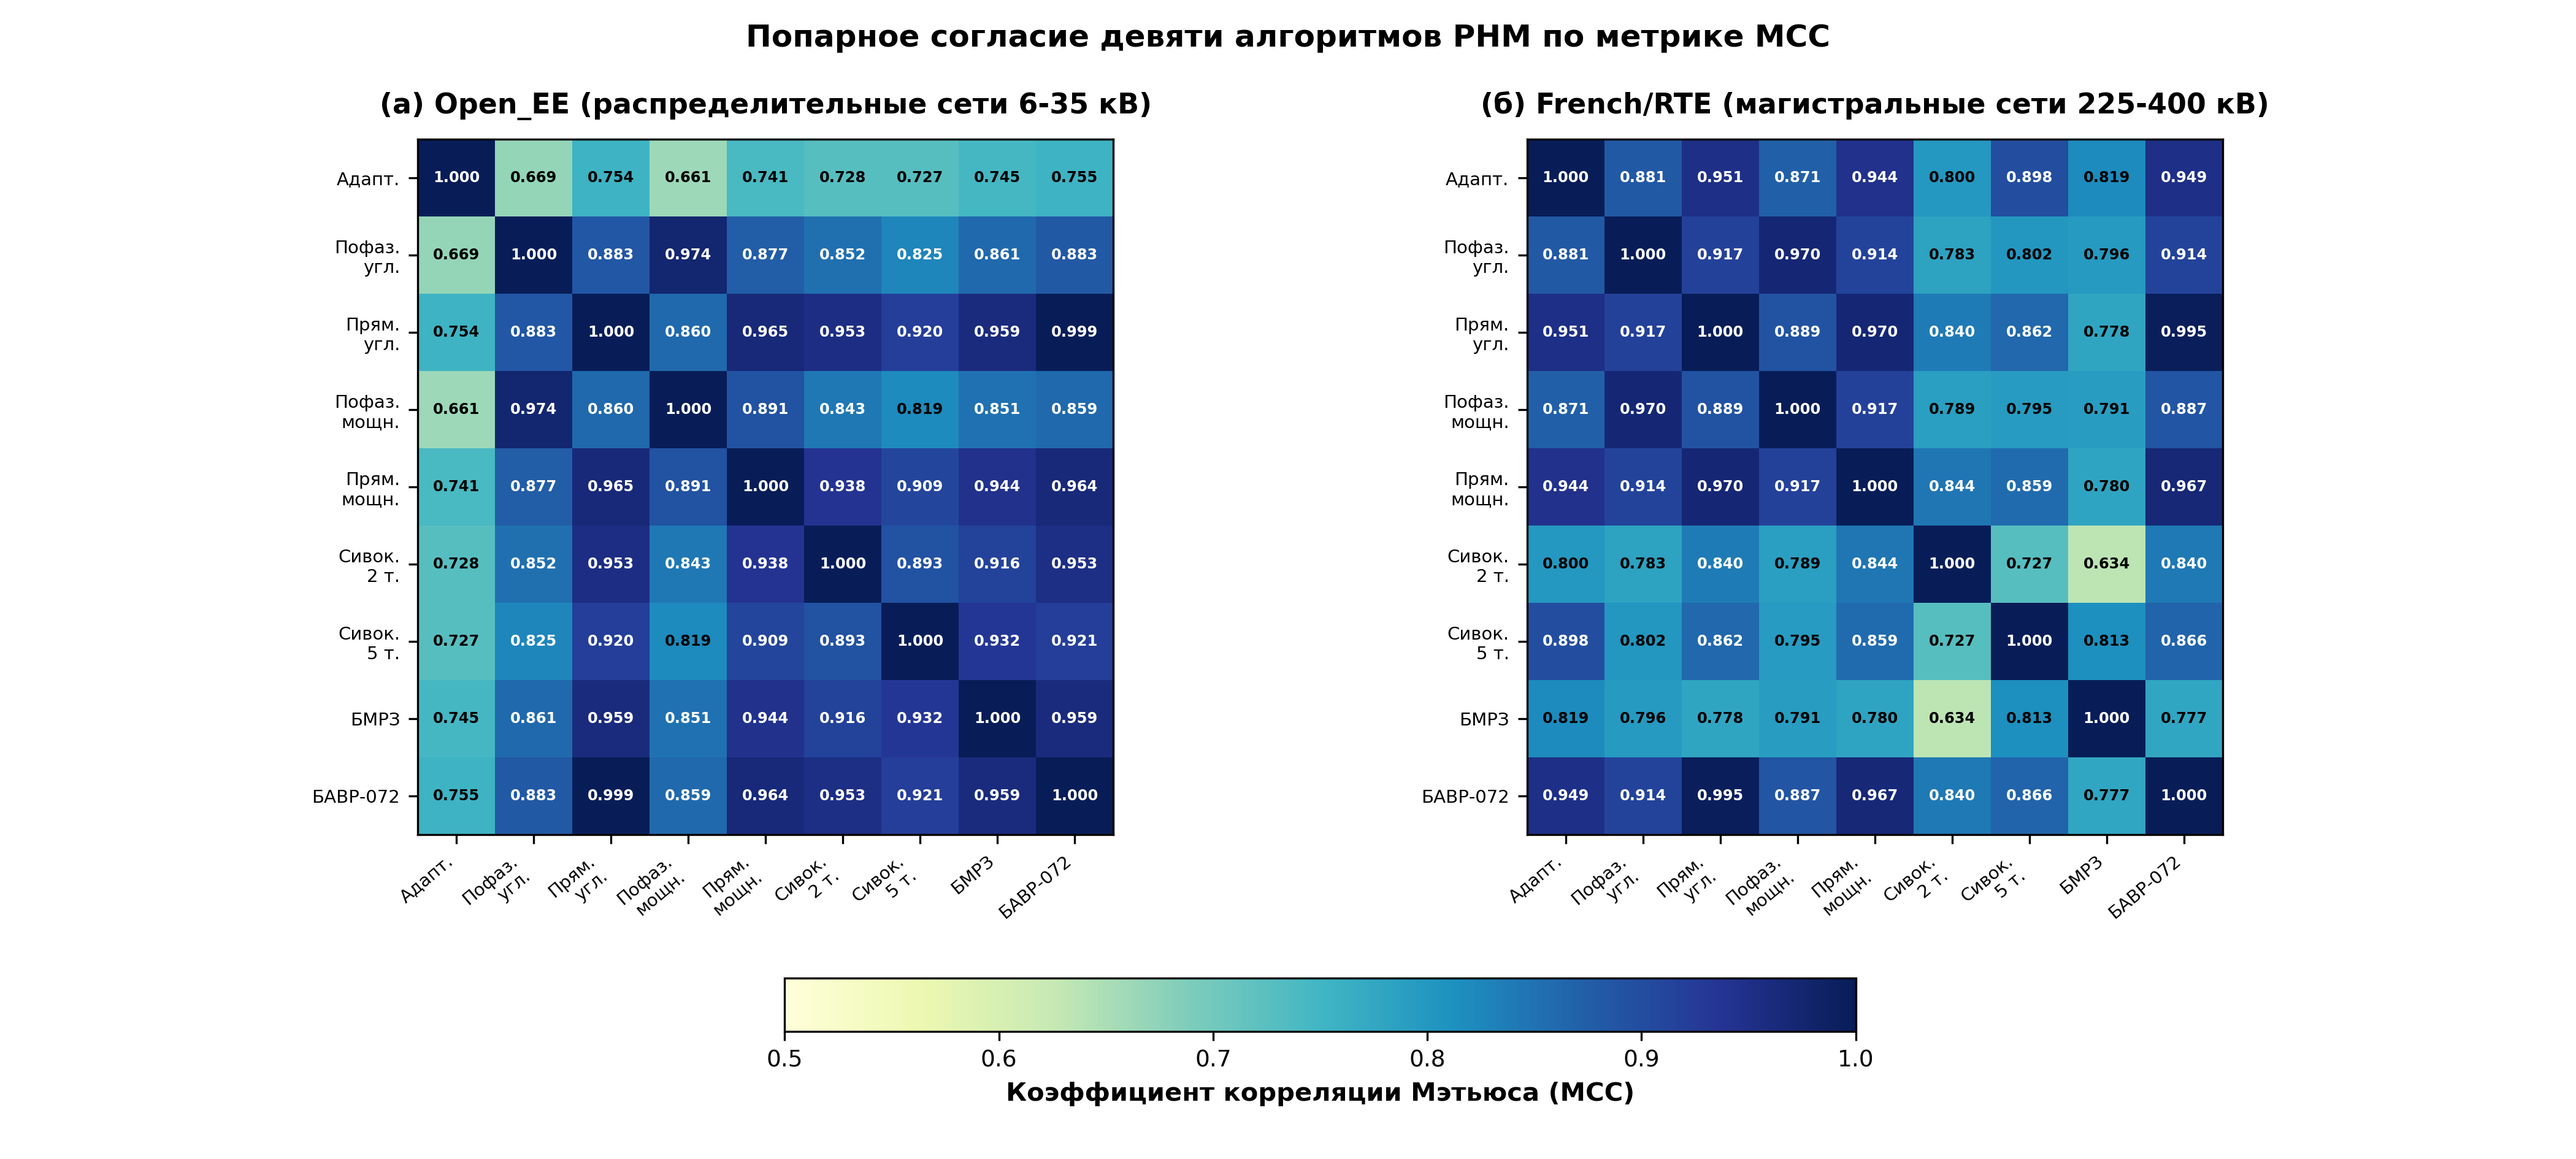
\includegraphics[width=\textwidth]{figures/ch05/ch05_pairwise_agreement_article.png}
\caption{Попарное согласие девяти органов РНМ
по коэффициенту MCC в двух источниках осциллограмм}
\label{fig:ch5_pairwise_agreement}
\figurereview{Исходный рисунок 4 статьи 5.
Для печати увеличить названия строк и столбцов.
БМРЗ и БАВР-072 здесь обозначают рассмотренные адаптации,
а не исчерпывающее испытание промышленных устройств.}
\end{figure}

Совместное решение девяти органов кодируется
последовательностью девяти двоичных признаков.
Сначала расположен адаптивный орган,
затем фазный угловой, угловой прямой последовательности,
фазный мощностной и мощностной прямой последовательности.
Далее следуют двухвыборочный, пятивыборочный,
БМРЗ и адаптация БАВР-072.
Единица обозначает прямое направление,
ноль отсутствие такого признака.
Сочетания учитываются только на общей
применимой части всех девяти ответов.
Неопределённое направление не подменяется нулём.

Полное совпадение прямых решений
занимает 40,33\% таких отсчётов Open\_EE
и 43,46\% French/RTE.
Полное совпадение нулевых ответов
занимает соответственно 36,09 и 34,20\%.
Вместе это 76,42 и 77,66\% общих ответов.
Изолированное прямое решение адаптивного органа
составляет 11,00\% в Open\_EE
и менее 1\% во French/RTE.

Нулевой ответ здесь означает результат
принятой характеристики с её порогами.
Он не доказывает отрицательной активной мощности
в каждом соответствующем отсчёте.
Полный консенсус также не превращается
в автоматически правильное действие автоматики.
Практически важны как записи с расхождением,
так и случаи, где несколько близких характеристик
могут иметь одно общее ограничение.

Распределение сочетаний показано
на рисунке~\ref{fig:ch5_state_patterns}.
Общие применимые отсчёты всех девяти органов
имеются в 34\,379 записях Open\_EE
и 11\,789 записях French/RTE.
Остальные записи не получают искусственную
комбинацию из нулей.

\begin{figure}[htbp]
\centering
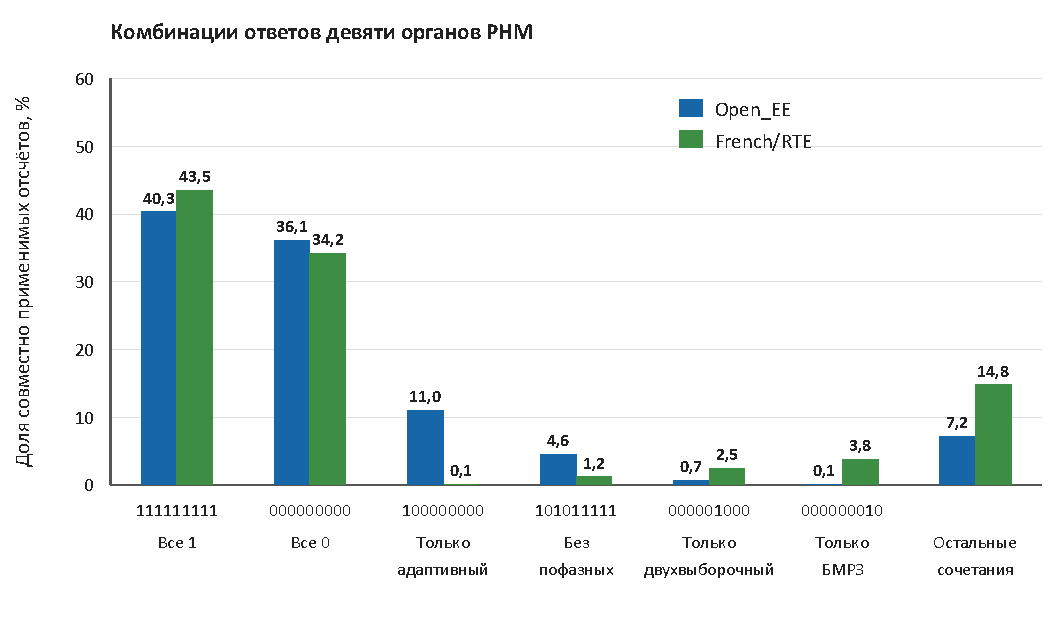
\includegraphics[width=\textwidth]{figures/ch05/ch05_state_patterns.pdf}
\caption{Комбинации ответов девяти РНМ
на общей применимой части.
Доли рассчитаны по отсчётам}
\label{fig:ch5_state_patterns}
\end{figure}
\figurereview{Идея исходного рисунка 5 статьи 5.
Векторный график построен по сохранённому
algorithm\_state\_patterns.csv, поле point\_fraction.
Исправлена неверная трактовка ординаты как физического времени.
Новых сигналов, расчётов органов или разметки нет.
Значения и порядок битов проверены по первичному CSV.}

\subsection{Различия источников и многомерная структура записей}
\label{sec:ch5_population_structure}
\conceptsource{Статья 5, подразделы 6.6--6.7, 7.7--7.8
и рисунок 6. Интегральный профиль осциллограммы
отличается от спектрального входа нейросетевого РНМ.}

Состав двух архивов дополнительно рассматривается
по обобщённому описанию каждой осциллограммы.
В него входят уровни токов и напряжений,
несимметрия, пик-факторы, характеристики регистрации
и распределение ответов измерительных органов.
Это признаки записи целиком,
а не входной спектральный срез нейросети.
Перед анализом пропуски заполняются медианами,
сильно асимметричные величины логарифмируются,
масштабы согласуются по межквартильному размаху.

\iffalse
(Примечание автора: Надо бы пояснить, что такое главная компонента и зачем мы её смотрим. Чем она полезна и зачем ввели, а то как будто прост пихнули, чтобы добавить что-то.)
(Примечание автора: Ок, закрываем задачу.)
\fi
\authorreviewnote{AA176}

Метод главных компонент позволяет кратко показать различия
между записями, описанными сразу несколькими признаками.
Вместо множества осей строятся новые оси, вдоль которых записи
различаются сильнее всего. Такая проекция помогает увидеть
отдельные группы и проверить, представлены ли они при отборе
материала для разметки. Она не определяет направление мощности.

Под MCC понимается коэффициент согласованности двух двоичных
решений с учётом совпадений и ошибок обоих направлений.
Значение, близкое к единице, означает согласованные ответы,
около нуля указывает на слабую связь, отрицательное значение
на преимущественно противоположные решения. Здесь он помогает
найти пары органов, различия которых стоит рассмотреть на записях.

Проекция главных компонент приведена
на рисунке~\ref{fig:ch5_population_pca}.
Первая компонента объясняет 50,71\% дисперсии
и преимущественно связана с уровнем напряжения.
Две компоненты вместе сохраняют 69,37\%,
четыре 82,99\%.
Следовательно, двумерная проекция показывает
существенную, но неполную часть различий.
Расстояние между точками не определяет
правильное направление мощности или требуемую команду БАВР.

\begin{figure}[p]
\centering
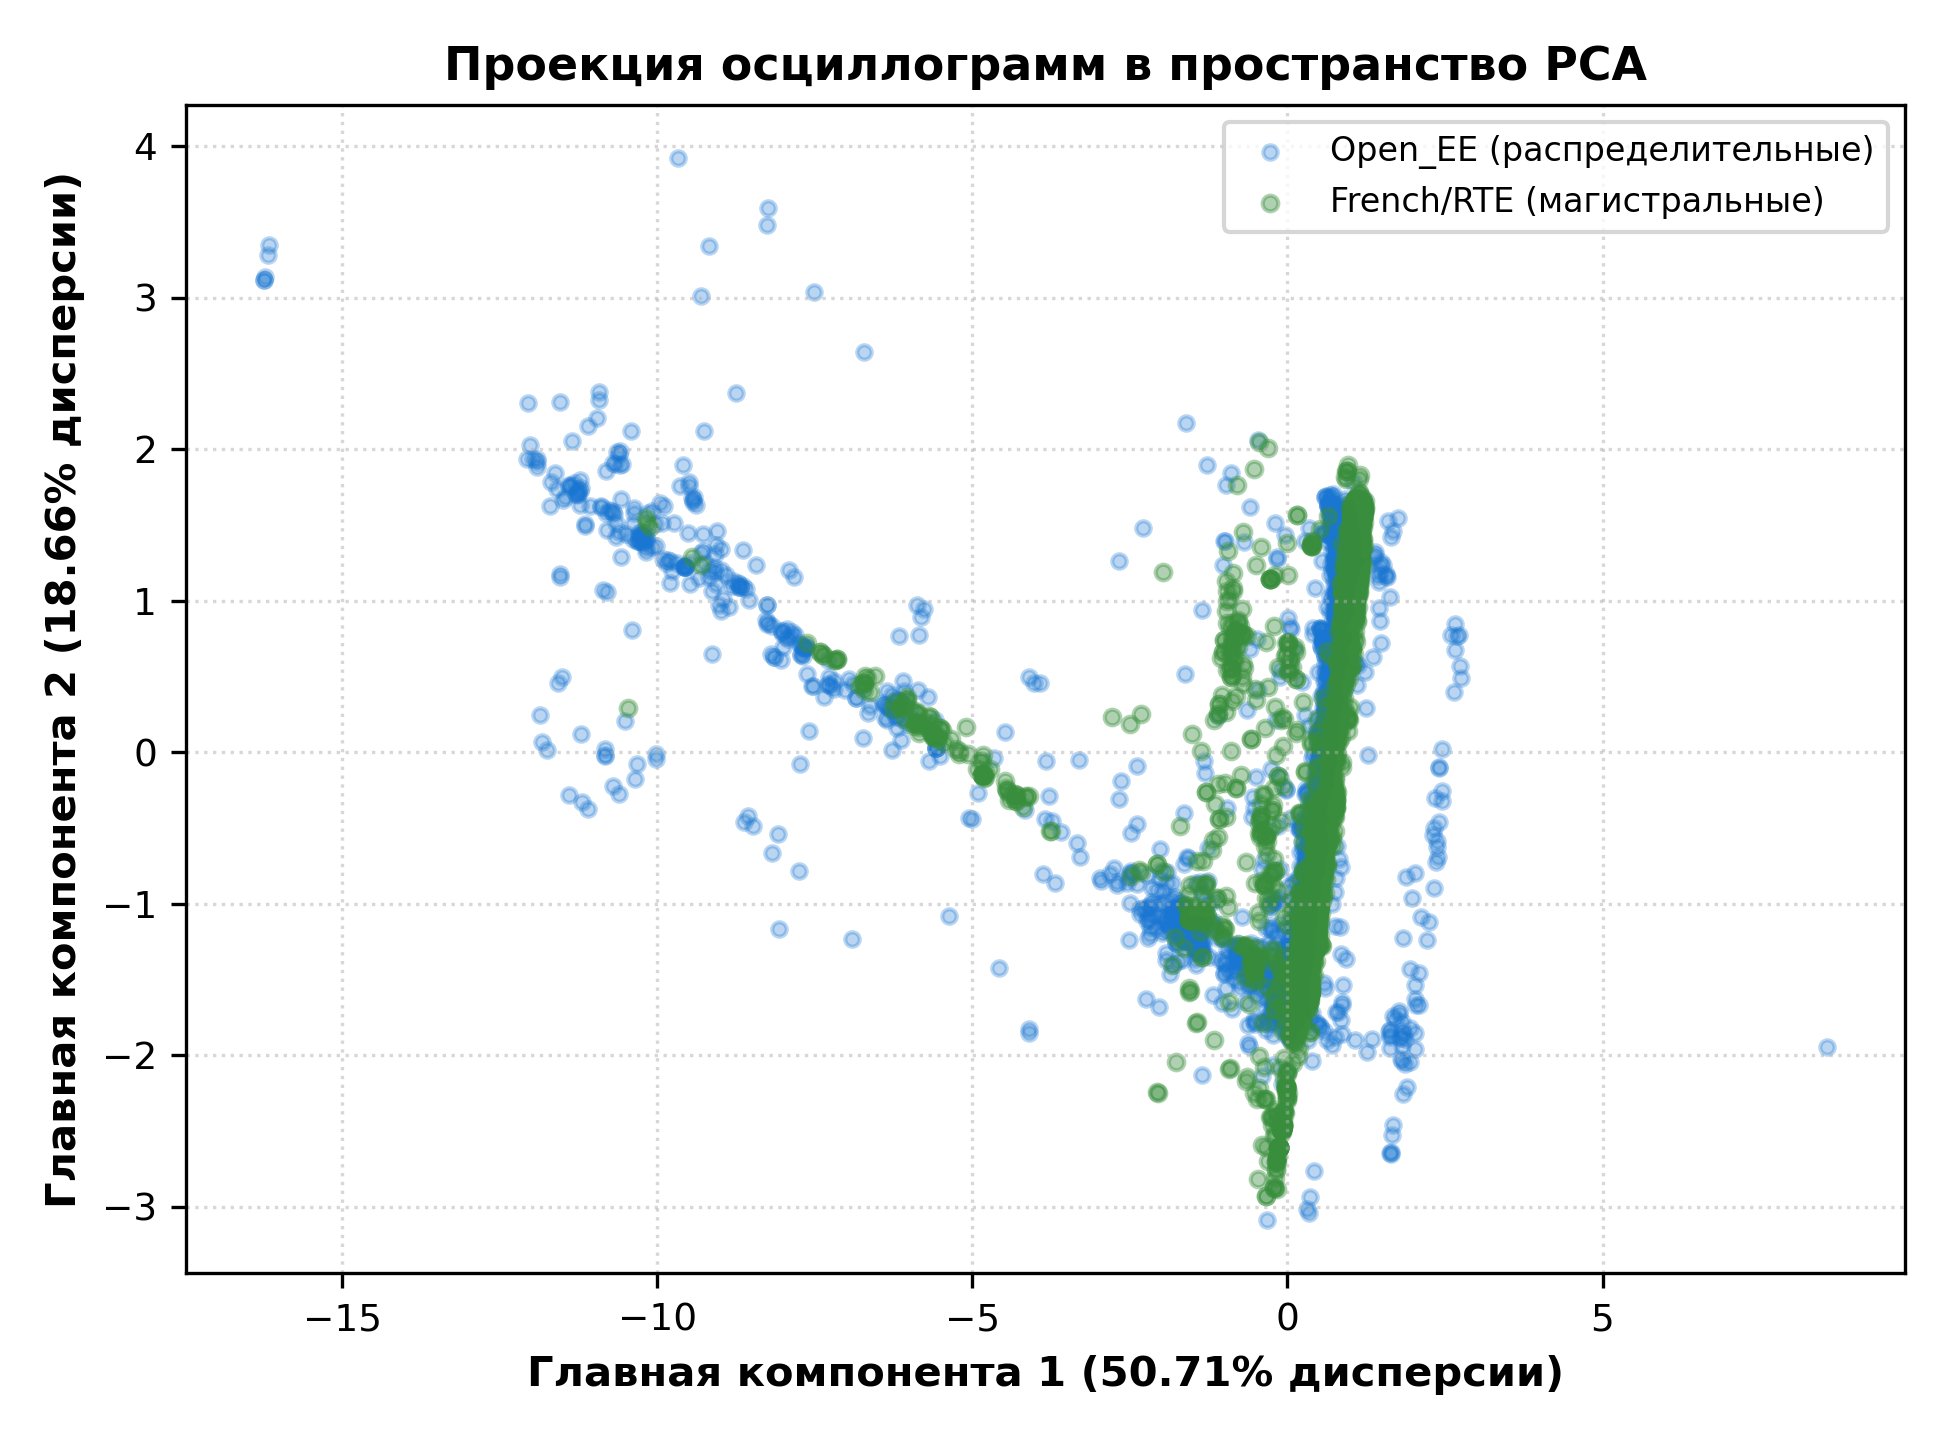
\includegraphics[width=0.76\textwidth]{figures/ch05/ch05_pca_projection_article.png}
\par\medskip
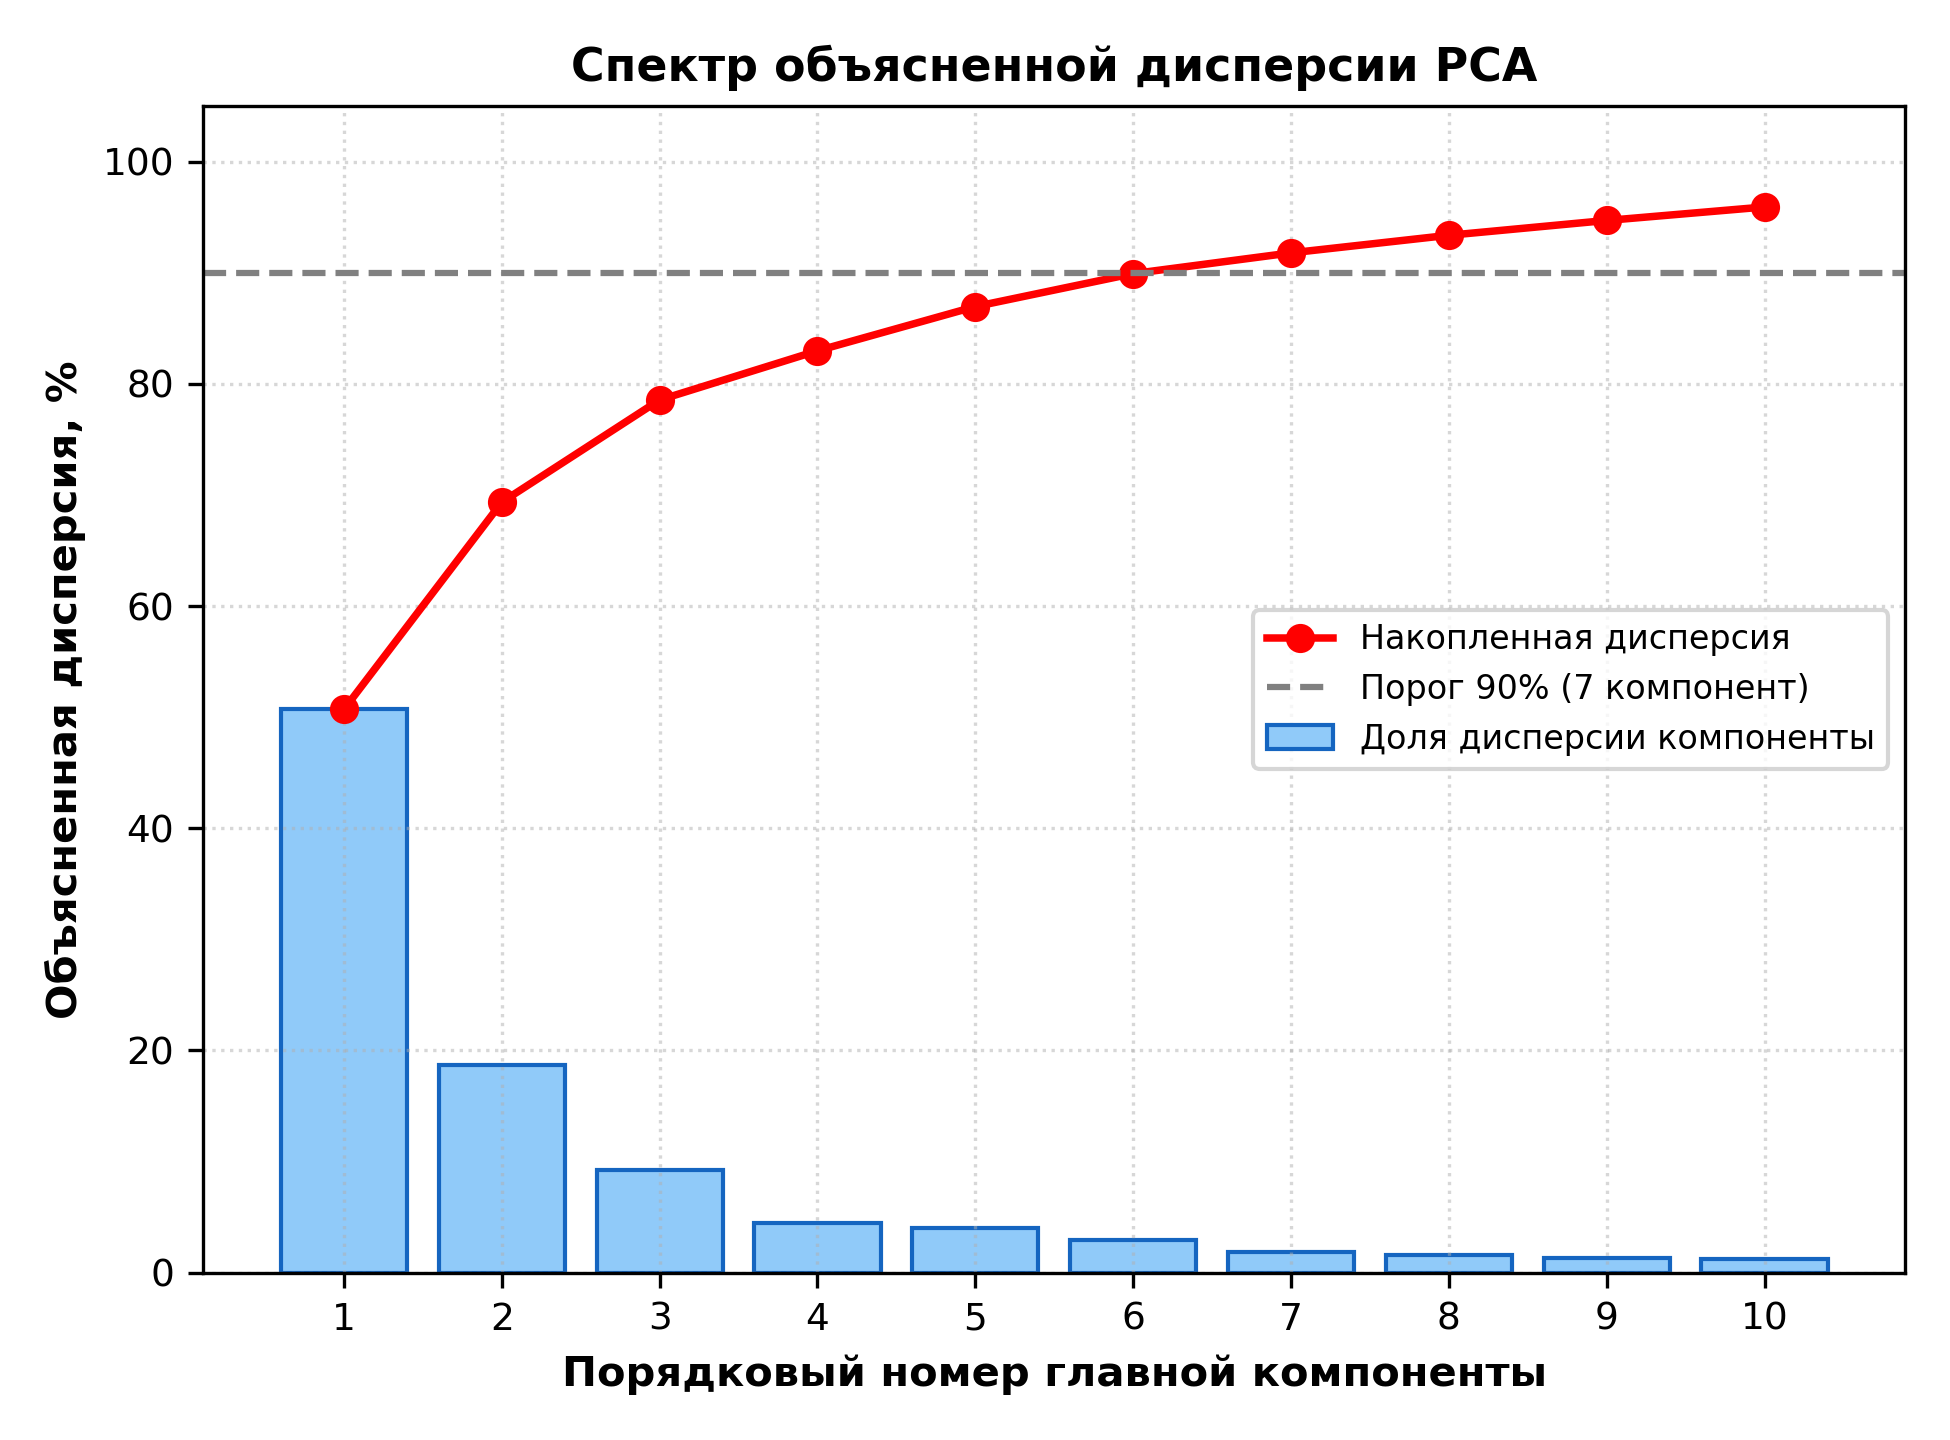
\includegraphics[width=0.76\textwidth]{figures/ch05/ch05_pca_variance_article.png}
\caption{Проекция интегральных профилей осциллограмм
на первые две главные компоненты и спектр
объяснённой дисперсии}
\label{fig:ch5_population_pca}
\figurereview{Исходные отдельные панели 6а и 6б из материалов
статьи, без перестроения. Они использованы вместо общего
рисунка с неточным заголовком о спектральных признаках.
Генератор показывает до 5000 записей каждого источника,
а не 4000 суммарно, как написано в одном абзаце статьи.
Эта проекция служит описанием массива, не классификацией повреждений.}
\end{figure}

Группировка похожих записей во French/RTE
выделяет две хорошо отделённые группы,
включая 259 записей с почти нулевыми токами и напряжениями.
Для Open\_EE разбиение на три группы
устойчиво к повторной инициализации,
но разделение существенно слабее.
Две крупные группы содержат 45,46 и 48,52\% записей,
малая низкоэнергетическая 6,02\%.
Такая устойчивость означает воспроизводимость группировки,
а не доказательство существования трёх физических классов.
Группы полезны для проверки охвата материала
и выбора осциллограмм для экспертного рассмотрения.

\iffalse
(Примечание автора: Не совсем понятно к чему применили ROC-AUC? К частоте АЦП или сети? Ну тогда понятно дело, что они разные… В общем вопрос остаётся, да и так же как и раньше – зачем всё это?.)
(Примечание автора: Ок, закрываем задачу.)
\fi
\authorreviewnote{AA177}

В диагностике источника целевая метка означает принадлежность
записи одному из двух архивов. Сначала проверяется, насколько
их можно различить по физическим признакам, затем учитываются
параметры регистрации. Это позволяет обнаружить ситуацию,
когда модель различает технические особенности архивов.
Поэтому высокая оценка этого опыта служит основанием проверять
результаты отдельно по источникам, а не показателем качества РНМ.

В отдельном диагностическом сравнении
источник записи восстанавливается по физическим признакам
с ROC-AUC, равной 0,850.
После добавления параметров регистрации она достигает 0,99985.
Этот результат показывает выраженные различия двух массивов,
в том числе технические особенности АЦП.
Он не позволяет объяснить их одной физической причиной
или переносить высокую различимость источников
на качество самого РНМ.
Поэтому результаты измерительных органов
далее рассматриваются для каждого источника отдельно.

\clearpage
\subsection{Сопоставление с экспертным направлением}
\conceptsource{Статья 5, таблица 10 и пояснения
валидационной сетки. Сохранены разные n направления
при общей исходной сетке.}

\iffalse
(Примечание автора: Чё? Так мало? Всего лишь? Эмм… Так может нам перезапустить на большем числе размеченных данных? Ведь уже есть.. Хотя понял, валидационные. Но погодь, можно же все, зачем тут только валидационные? Мы же не нейронку проверяем которую учили. Ну можно и разбить данные на «всё» и «валидационное».)
\fi
\authorreviewnote{AA178}

В исходном экспертном сопоставлении использованы
54 валидационные записи, из них 32 Open\_EE
и 22 French/RTE.
Общая сетка содержит 12\,942 точки применимости,
в 10\,181 из которых эксперт определил направление.
Внутри файла применяется шаг пять отсчётов
и ограничение 256 точками.
Это уменьшает преобладание длинных записей,
но не превращает соседние точки
в независимые аварийные события.

Начальное накопление контекста и переходная
маска в этой сетке исключены.
Направление оценивается при совместной применимости
эксперта и проверяемого органа.
Поэтому фактическое число сравниваемых точек
различается, как показано в
таблице~\ref{tab:ch5_analytical_expert}.
Неприменимые ответы оцениваются отдельно,
а не засчитываются правильным направлением.

\begin{table}[htbp]
\centering\small
\caption{Аналитические РНМ на исходной экспертной
валидационной сетке}
\label{tab:ch5_analytical_expert}
\begin{tabularx}{\textwidth}{@{}Xrrr@{}}
\toprule
Орган & Точек направления & Macro-F1, \% & MCC \\
\midrule
Адаптивный & 10\,176 & 89,59 & 0,794 \\
Пофазный угловой & 10\,008 & 44,79 & 0,037 \\
Угловой прямой последовательности & 9998 & 58,17 & 0,231 \\
Пофазный мощностной & 10\,008 & 46,10 & 0,159 \\
Мощностной прямой последовательности & 9998 & 55,57 & 0,279 \\
Двухвыборочный & 10\,013 & 52,77 & 0,153 \\
Пятивыборочный & 10\,089 & 58,73 & 0,325 \\
БМРЗ, дополнительная ветвь & 9998 & 65,62 & 0,484 \\
Адаптация БАВР-072 & 10\,157 & 58,68 & 0,241 \\
\bottomrule
\end{tabularx}
\end{table}

\iffalse
(Примечание автора: И непонятно что такое MCC, если не описывалось где-то ,может забыл.)
(Примечание автора: Ок, закрываем задачу.)
\fi
\authorreviewnote{AA179}

MCC учитывает четыре исхода двоичного сравнения.
Единица означает полное совпадение,
ноль отсутствие выявленной связи ответов с эталоном.
Macro-F1 одинаково учитывает два направления.
Оба показателя описывают принятую сетку
и правила допуска к сравнению.
Они дополняются проверкой полного состояния
и ошибочного времени из
раздела~\ref{sec:ch5_engineering_verification}.

На этой сетке адаптивный орган имеет
наибольшее согласие направления с экспертом.
Но объединённый результат скрывает различия источников.
Для пятивыборочного органа Macro-F1
составляет 94,67\% во French/RTE
и 28,67\% в Open\_EE.
Для БМРЗ-варианта получены 89,84 и 46,89\%.
Такое расхождение важно для выбора
направления модернизации применительно
к промышленному БАВР.
Оно требует разбора режимов и целевой логики,
а не только выбора максимального числа
в объединённой таблице.

Эта проверка показывает, как массовое сравнение
переходит к предметной оценке конкретного органа.
Высокое согласие в одном источнике
не освобождает от проверки другого,
а изменение формулы проверяется
по тем же требованиям к выходу.
Дальнейшее сравнение с обучаемыми моделями
сохраняет эти единицы оценки и ограничения.


